\chapter{検定}\label{ch:testing}

\ref{ch:parameter_est}章までで、多項ロジットモデルを作って各選択肢の選択確率を求めることができるようになりました。

しかし、最尤推定法によって尤もらしいパラメータを推定することができたからといって、そのパラメータが統計的に信頼できるとは限りません。また、そのパラメータと説明変数を持つモデルが実際のデータにどのくらいうまく適合しているかも知る必要があります。

例えば、もし所要時間の重みパラメータ $\beta_{time}$ の推定値が統計的に信頼できないとみなすならば、そのモデルを使って所要時間の変化に伴う乗客数の変化を推定することはできません。また、新しい説明変数とパラメータを追加することでモデルの適合度が\textbf{有意に}向上するのであれば、新しいモデルの方を採用するべきでしょう。

求めたパラメータが統計的に信頼できるかどうかを判定するための方法の一つとして、\textbf{t検定}がしばしば用いられます。また、モデルと実際のデータの適合度合いを見るために\textbf{尤度比検定}が用いられます。

\section{t検定}\label{sec:t_test}

ここでは、紛らわしい統計用語を順を追って整理し、最終的にt検定について説明します。

\subsection{統計量}\label{ssec:statistic}

統計的分析の対象となる人や物事の集まりを\textbf{母集団}、母集団から抽出してきた人や物事の集まりを\textbf{標本}といいます。標本に対して、標本に関する何らかの値(選択行動の結果など)を取り出してくると、その値は標本の選び方によって変わる\textbf{確率変数}になります。このようにして得られる確率変数の集まりのことを\textbf{標本変量}といいます。

\textbf{統計量}とは、標本変量に対して何らかの操作を行うことによって得ることができる、その標本変量の特徴を簡潔に示す量のことです。例えば算術平均は「標本変量の総和を標本数で割る」という操作によって得ることができる統計量です。また分散、中央値、最頻値なども同様に統計量です。

重要な事実として、標本変量は確率変数の集まりなので、それに対して操作を加えて得られる\textbf{統計量もまた確率変数}です。

\subsection{推定値と推定量}\label{ssec:estimator}

\ref{sec:likelihood}節では最尤推定法によって未知パラメータ $\bm\beta$ の値を推定しました。このときは実際に観測されたデータを使って推定を行ったので $\bm\beta$ の具体的な値を求めることができました。これを $\beta$ の\textbf{推定値}と呼びます。特にこの場合は最尤推定法によって得られた値なので、\textbf{最尤推定値}と呼びます。しかし、最尤推定値の値は標本の選び方によって変わるはずです。

最尤推定の結果は、標本変量に対して尤度を最大化するという操作を行うことで得られる量なので、統計量の定義を満たしています。このように、何らかの推定のために得る統計量のことを\textbf{推定量}と呼び、$\hat\beta$ と記します。特にこの場合は最尤推定法によって得られた推定量なので、\textbf{最尤推定量}と呼びます。最尤推定量は統計量なので確率変数であり、したがって確率分布を持ちます。

t検定では、「各パラメータの最尤推定量がとる値が $0$ になる確率」を計算します。$i$ 番目のパラメータ $\beta_i$ の真の値が $0$ であるとき、そのパラメータに対応する説明変数 $x_i$ に何を代入しても効用の値が変化しないので、その説明変数は選択行動を説明するのに全く役立たないということになります。逆にこのようなことになる確率が十分に低ければ、そのパラメータに対応する説明変数 $x_i$ は選択行動を説明しているということができます。

なお、最尤推定量は以下の性質を満たします。

\begin{description}
    \item[一致性] 無限個の標本を用いて推定した最尤推定値は、パラメータの真値に一致する。
    \item[漸近正規性] 標本が多く\footnote{50件とか100件以上などと言われています。}なると、最尤推定量の分布は正規分布に近づく。
    \item[漸近有効性] 標本が多くなると、最尤推定量の分散は\textbf{クラメール・ラオの不等式}の下限に近付く。
\end{description}

\subsection{最尤推定量の分散}\label{ssec:variance_estimator}

推定量の期待値がパラメータの真値に一致するとき、その推定量は\textbf{不偏推定量}であるといいます(一致性とは異なる概念です)。さらに、その不偏推定量が他のどの不偏推定量よりも分散が大きくないとき、その推定量は\textbf{有効推定量}であるといいます。最尤推定量は不偏推定量ではないので、当然有効推定量でもありませんが、標本が多くなると漸近的に有効推定量のようなふるまいを見せる、というのが漸近有効性です。

有効推定量が定義可能であることからも分かるように、不偏推定量の分散には下限が存在します。この不偏推定量の分散の下限を示すのがクラメール・ラオの不等式です。

\begin{theorem}[クラメール・ラオの不等式]
    \label{it:cramer_rao}
    $\bm{\hat\beta}$ をパラメータ $\bm\beta$ の不偏推定量とし、$\cov(\bm{\hat\beta})$ は $\bm{\hat\beta}$ の分散共分散行列、$LL$ は対数尤度関数とする。このとき以下の行列に対する不等式が成り立つ。
    
    \begin{align}
        \label{eq:fisher_information}
        I(\bm\beta) \coloneqq -E\left[\nabla\nabla^\top LL(\bm\beta)\right] \\  
        \label{eq:cramer_rao}
        \cov(\bm{\hat\beta}) \ge I(\bm\beta)^{-1}
    \end{align}
    ただし、式(\ref{eq:cramer_rao})の不等号は、左辺から右辺を引いた行列 $\cov(\bm{\hat\beta})-I(\bm\beta)^{-1}$ が半正定値行列であることを意味する\footnote{もし $\bm\beta$ が1変数のパラメータであれば、この不等号は単に実数の不等号と同じ意味になります。}。
\end{theorem}
\begin{proof}
    \ref{prf:cramer_rao}を参照。
\end{proof}

$I(\bm\beta)$は\textbf{フィッシャー情報行列}と呼ばれます。なお、$\nabla\nabla^\top LL(\bm\beta)$ は書き出すと下の式(\ref{eq:hessian_matrix})のようになり、特に行列部分には\textbf{ヘッセ行列}という名前がつけられています。

\begin{equation}
    \label{eq:hessian_matrix}
    \nabla\nabla^\top LL(\bm\beta) = \begin{bmatrix}
        \frac{\partial^2 LL}{\partial {\beta_1}^2}              & \frac{\partial^2 LL}{\partial \beta_1 \partial \beta_2} & \cdots & \frac{\partial^2 LL}{\partial \beta_1 \partial \beta_n}  \\
        \frac{\partial^2 LL}{\partial \beta_2 \partial \beta_1} & \frac{\partial^2 LL}{\partial {\beta_2}^2}              & \cdots & \frac{\partial^2 LL}{\partial \beta_2 \partial \beta_n } \\
        \vdots                                                  & \vdots                                                  & \ddots & \vdots                                                   \\
        \frac{\partial^2 LL}{\partial \beta_n \beta_1}          & \frac{\partial^2 LL}{\partial \beta_n \partial \beta_2} & \cdots & \frac{\partial^2 LL}{\partial {\beta_n}^2}
    \end{bmatrix} \bm\beta
\end{equation}

等号が成立する時、$\bm{\hat\beta}$ は分散の下限を達成しているので、$\bm{\hat\beta}$ は有効推定量となります。最尤推定量の場合は、漸近有効性により、標本が十分多ければ等号成立、すなわち

\begin{equation}
    \label{eq:fisher_information_inv}
    \cov(\bm{\hat\beta}) \simeq I(\bm\beta)^{-1}
\end{equation}

としてよいです。このように、フィッシャー情報行列を求めることで、最尤推定量の分散を求めることができます。

フィッシャー情報行列を確率変数である$\bm\beta$の分布から直接計算することもできますが、フィッシャー情報行列に代えて\textbf{観測された情報行列}を用いる方が計算が簡単かつ有用です\cite{Efron1978}。観測された情報行列$J(\bm{\hat\beta})$は次のように定義されます。

\begin{equation}
    \label{eq:observed_information}
    J(\bm{\hat\beta}) \coloneqq -\nabla\nabla^\top LL(\bm{\hat\beta})
\end{equation}

式(\ref{eq:observed_information})を用いると、式(\ref{eq:fisher_information_inv})の代わりに次の式が得られます。

\begin{equation}
    \label{eq:observed_information_inv}
    \cov(\bm{\hat\beta}) \simeq J(\bm{\hat\beta})^{-1}
\end{equation}

\subsection{区間推定}\label{ssec:interval_est}

t検定では、各パラメータについて、次のような\textbf{帰無仮説}を立てます。

\begin{itembox}[l]{t検定での帰無仮説}
    パラメータ $\beta_i$ の最尤推定量 $\hat\beta_i$ がとる値は $0$ である。
\end{itembox}

この帰無仮説が一定の\textbf{有意水準}で\textbf{棄却}されるならば、パラメータ $\beta_i$ の最尤推定量が $0$ とは有意に異なるとみなすことができます。

帰無仮説が棄却されるかどうかを調べるためには、$\beta_i$ の最尤推定量がとりうる区間を推定し、$0$ が\textbf{信頼区間}内に入ってこないことを確認すればよいです。

\begin{figure}[ht]
    \centering
    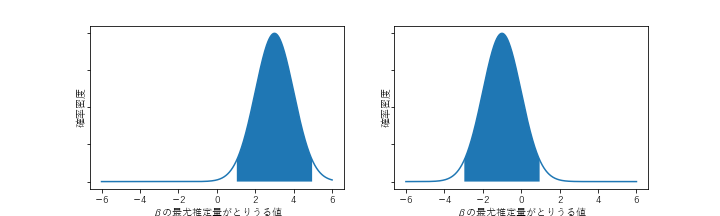
\includegraphics[width=0.9\hsize]{figure/interval_estimation.png}
    \caption{信頼区間}
    \label{fig:interval_est}
\end{figure}


図\ref{fig:interval_est}で青く塗っている区間が信頼区間です。例えば「$95\%$ 信頼区間」であれば、パラメータ $\beta_i$ の最尤推定量 $\hat\beta_i$ がとる値が $95\%$ の確率でその区間内に収まることを意味します。

左の図では、$95\%$ 信頼区間内に $0$ が含まれていないので、$\hat\beta_i$ が取る値が $0$ になる確率は $5\%$ 以下となります。すると「パラメータ $\beta_i$ の最尤推定量 $\hat\beta_i$ がとる値は $0$ である」という帰無仮説は $5\%$ 有意水準で棄却されることになり、そのパラメータに対応する説明変数は選択行動を説明しているということができます。

いっぽう右の図では、$95\%$ 信頼区間内に $0$ が含まれているので、帰無仮説は棄却されません。すると、そのパラメータに対応する説明変数が選択行動を説明しているかどうかは分かりません(\textbf{説明変数が「効かない」ことを意味しているわけではなく、「効くとは言い切れない」ということを意味します})。

ここで、信頼区間の幅を求めるには、最尤推定量の分散が必要になります。最尤推定量の分散を求めるために式(\ref{eq:observed_information_inv})を用います。なお$L$ のヘッセ行列は数値微分によって計算できます。

各パラメータの最尤推定量の分散 $\bm s^2$ が分かれば、最尤推定量の漸近正規性により、正規分布の場合と同様に信頼区間を求めることができます。

各パラメータの最尤推定量を $t_i\coloneq\frac{\hat\beta_i}{s}$ と標準化します。このとき出現する値 $t_i$ は\textbf{t値}と呼ばれ、t値が\textbf{標準正規分布}の $95\%$ 信頼区間内に入っていないならば、帰無仮説は $5\%$ 有意水準で棄却されることになります。このようなt値の閾値は $|t|>1.96$ です(標準正規分布の両側 $5\%$ 点は $1.96$)。また、$|t|>2.58$ となれば帰無仮説は $1\%$ 有意水準で棄却されることになります。

\section{尤度比指標}\label{sec:likelihood_ratio}

\subsection{尤度比検定}

尤度比検定は、先ほどのt値とは異なり、あるモデルが全体として別のモデルより適合度が高いかどうかを見る検定です。

モデルAを、モデルBにいくつかの説明変数とパラメータを加えたモデルとします。モデルAとモデルBの尤度比は、文字通り尤度の比 $\frac{L(\bm{\hat\beta_A})}{L(\bm{\hat\beta_B})}$ です。尤度比の対数は $LL(\bm{\hat\beta_A})-LL(\bm{\hat\beta_B})$ となり、対数を取った方の値を単に\textbf{尤度比}と呼ぶことがあります。尤度比は確率変数なので検定可能です。

尤度比検定では、次のような帰無仮説を立てます。

\begin{itembox}[l]{尤度比検定での帰無仮説}
    帰無仮説:モデルAとモデルBの尤度比は $0$ である。
\end{itembox}

尤度が大きい方がより「もっともらしい」モデルなので、説明変数が多いモデルAの方が尤度が大きくなってほしいところです。この帰無仮説が棄却されればモデルAの方が有意に尤度が大きいということができ、二つのモデルの適合度の差が有意なものであるということができます。

ところで、標本が十分多いとき、尤度比を $2$ 倍した値は\textbf{カイ二乗分布}と呼ばれる分布に従うことが知られています。特に、$\bm\beta_A$ のパラメータ数が $N_A$ 個、$\bm\beta_B$ のパラメータ数が $N_B$ 個であるとき、 $2(LL(\bm{\hat\beta_A})-LL(\bm{\hat\beta_B}))$ は\textbf{自由度} $N_A-N_B$ のカイ二乗分布に従います。

したがって、帰無仮説「モデルAとモデルBの尤度比は $0$ である」を棄却するには、$2(LL(\bm{\hat\beta_A})-LL(\bm{\hat\beta_B}))$ の信頼区間内に $0$ が入ってこないことを示せばよいです。

たとえば $N_A=7, N_B=5$ のとき、自由度 $2$ のカイ二乗分布の上側 $5\%$ 点は $5.99$ なので、$2(LL(\bm{\hat\beta_A})-LL(\bm{\hat\beta_B}))>5.99$ ならば $5\%$ 有意水準で帰無仮説が棄却されることになります。

特に、すべての選択肢の効用を $0$ としたモデル(説明変数もパラメータもないモデル)をモデルBとして尤度比検定することで、作ったモデルの適合度が有意であることを確認することができます。すべての選択肢の効用を $0$ としたモデルのことを \textbf{Null model} と呼び、その対数尤度は $LL(\bm 0)$ で求めることができます。

注意すべき点として、モデルAはモデルBを含んでいる、上位互換のモデルである必要があります。厳密に述べると、モデルAに含まれない説明変数・パラメータであって、モデルBに含まれるような説明変数・パラメータがあってはいけません。

\subsection{McFaddenの擬似決定係数}

尤度比検定では、尤度比をカイ二乗分布の上側 $5\%$ 点と比較することで、モデルの適合度が有意であるかどうかを判定しました。しかし、カイ二乗分布の上側 $5\%$ 点は自由度によって変化するので、モデルの適合度が有意であるかどうかを判定するためには、モデルのパラメータ数に応じてカイ二乗分布の上側 $5\%$ 点を求める必要があります。回帰分析における決定係数のように、0から1の範囲に収まるより分かりやすい指標が欲しいところです。

そこで、\textbf{McFaddenの擬似決定係数}という指標が考案されました。McFaddenの擬似決定係数 $\rho^2$ は次のように定義されます。

\begin{equation}
    \rho^2 \coloneq \frac{LL(\bm 0)-LL(\bm{\hat\beta})}{LL(\bm 0)} = 1-\frac{LL(\bm{\hat\beta})}{LL(\bm 0)}
\end{equation}

この指標は $0$ から $1$ の範囲に収まるので、決定係数のようにモデルの適合度を示す指標として使うことができます。交通分野で\textbf{尤度比}といった場合、このMcFaddenの擬似決定係数のことを指す場合もあります。

整理すると、単に尤度比といった場合、次の三つの値のどれを指しているかは資料によって異なります。

\begin{enumerate}
    \item 2つのロジットモデルの尤度の比 $\frac{L(\bm{\hat\beta_A})}{L(\bm{\hat\beta_B})}$
    \item 2つのロジットモデルの対数尤度の差 $LL(\bm{\hat\beta_A})-LL(\bm{\hat\beta_B})$
    \item あるロジットモデルのMcFadden擬似決定係数 $\rho^2=1-\frac{LL(\bm{\hat\beta})}{LL(\bm 0)}$
\end{enumerate}

\subsection{自由度調整済み決定係数}

McFaddenの擬似決定係数は、モデルのパラメータ数に応じてカイ二乗分布の上側 $5\%$ 点を求める必要がないという利点がありますが、モデルのパラメータ数が多くなるほど指標値が増加するという欠点があります。そこで、\textbf{自由度調整済み決定係数}という指標が考案されました。

自由度調整済み決定係数 $\bar\rho^2$ は次のように定義されます。

\begin{equation}
    \bar\rho^2 \coloneq 1-\frac{LL(\bm{\hat\beta})-N}{LL(\bm 0)}
\end{equation}

$N$は未知パラメータの数です。

この指標はパラメータの数にかかわらず用いることができ、経験的に$0.2$以上であれば十分、$0.15$以上でもまあ良しとされます。

なお、自由度調整済み決定係数のことを\textbf{修正済み決定係数}と呼ぶこともあります。

ロジットモデルの推定を行った論文では、初期尤度(Null Model の対数尤度)$LL(\bm 0)$、最終尤度 $LL(\bm{\hat\beta})$ とともに、McFaddenの擬似決定係数や自由度調整済み決定係数が報告されることが多いです。報告の形式についてはこのあとの\ref{sec:est_result}節を参照してください。